% Options for packages loaded elsewhere
\PassOptionsToPackage{unicode}{hyperref}
\PassOptionsToPackage{hyphens}{url}
\PassOptionsToPackage{dvipsnames,svgnames,x11names}{xcolor}
\documentclass[
]{article}
\usepackage{xcolor}
\usepackage[margin=1in]{geometry}
\usepackage{amsmath,amssymb}
\setcounter{secnumdepth}{-\maxdimen} % remove section numbering
\usepackage{iftex}
\ifPDFTeX
  \usepackage[T1]{fontenc}
  \usepackage[utf8]{inputenc}
  \usepackage{textcomp} % provide euro and other symbols
\else % if luatex or xetex
  \usepackage{unicode-math} % this also loads fontspec
  \defaultfontfeatures{Scale=MatchLowercase}
  \defaultfontfeatures[\rmfamily]{Ligatures=TeX,Scale=1}
\fi
\usepackage{lmodern}
\ifPDFTeX\else
  % xetex/luatex font selection
\fi
% Use upquote if available, for straight quotes in verbatim environments
\IfFileExists{upquote.sty}{\usepackage{upquote}}{}
\IfFileExists{microtype.sty}{% use microtype if available
  \usepackage[]{microtype}
  \UseMicrotypeSet[protrusion]{basicmath} % disable protrusion for tt fonts
}{}
\makeatletter
\@ifundefined{KOMAClassName}{% if non-KOMA class
  \IfFileExists{parskip.sty}{%
    \usepackage{parskip}
  }{% else
    \setlength{\parindent}{0pt}
    \setlength{\parskip}{6pt plus 2pt minus 1pt}}
}{% if KOMA class
  \KOMAoptions{parskip=half}}
\makeatother
\usepackage{color}
\usepackage{fancyvrb}
\newcommand{\VerbBar}{|}
\newcommand{\VERB}{\Verb[commandchars=\\\{\}]}
\DefineVerbatimEnvironment{Highlighting}{Verbatim}{commandchars=\\\{\}}
% Add ',fontsize=\small' for more characters per line
\usepackage{framed}
\definecolor{shadecolor}{RGB}{248,248,248}
\newenvironment{Shaded}{\begin{snugshade}}{\end{snugshade}}
\newcommand{\AlertTok}[1]{\textcolor[rgb]{0.94,0.16,0.16}{#1}}
\newcommand{\AnnotationTok}[1]{\textcolor[rgb]{0.56,0.35,0.01}{\textbf{\textit{#1}}}}
\newcommand{\AttributeTok}[1]{\textcolor[rgb]{0.13,0.29,0.53}{#1}}
\newcommand{\BaseNTok}[1]{\textcolor[rgb]{0.00,0.00,0.81}{#1}}
\newcommand{\BuiltInTok}[1]{#1}
\newcommand{\CharTok}[1]{\textcolor[rgb]{0.31,0.60,0.02}{#1}}
\newcommand{\CommentTok}[1]{\textcolor[rgb]{0.56,0.35,0.01}{\textit{#1}}}
\newcommand{\CommentVarTok}[1]{\textcolor[rgb]{0.56,0.35,0.01}{\textbf{\textit{#1}}}}
\newcommand{\ConstantTok}[1]{\textcolor[rgb]{0.56,0.35,0.01}{#1}}
\newcommand{\ControlFlowTok}[1]{\textcolor[rgb]{0.13,0.29,0.53}{\textbf{#1}}}
\newcommand{\DataTypeTok}[1]{\textcolor[rgb]{0.13,0.29,0.53}{#1}}
\newcommand{\DecValTok}[1]{\textcolor[rgb]{0.00,0.00,0.81}{#1}}
\newcommand{\DocumentationTok}[1]{\textcolor[rgb]{0.56,0.35,0.01}{\textbf{\textit{#1}}}}
\newcommand{\ErrorTok}[1]{\textcolor[rgb]{0.64,0.00,0.00}{\textbf{#1}}}
\newcommand{\ExtensionTok}[1]{#1}
\newcommand{\FloatTok}[1]{\textcolor[rgb]{0.00,0.00,0.81}{#1}}
\newcommand{\FunctionTok}[1]{\textcolor[rgb]{0.13,0.29,0.53}{\textbf{#1}}}
\newcommand{\ImportTok}[1]{#1}
\newcommand{\InformationTok}[1]{\textcolor[rgb]{0.56,0.35,0.01}{\textbf{\textit{#1}}}}
\newcommand{\KeywordTok}[1]{\textcolor[rgb]{0.13,0.29,0.53}{\textbf{#1}}}
\newcommand{\NormalTok}[1]{#1}
\newcommand{\OperatorTok}[1]{\textcolor[rgb]{0.81,0.36,0.00}{\textbf{#1}}}
\newcommand{\OtherTok}[1]{\textcolor[rgb]{0.56,0.35,0.01}{#1}}
\newcommand{\PreprocessorTok}[1]{\textcolor[rgb]{0.56,0.35,0.01}{\textit{#1}}}
\newcommand{\RegionMarkerTok}[1]{#1}
\newcommand{\SpecialCharTok}[1]{\textcolor[rgb]{0.81,0.36,0.00}{\textbf{#1}}}
\newcommand{\SpecialStringTok}[1]{\textcolor[rgb]{0.31,0.60,0.02}{#1}}
\newcommand{\StringTok}[1]{\textcolor[rgb]{0.31,0.60,0.02}{#1}}
\newcommand{\VariableTok}[1]{\textcolor[rgb]{0.00,0.00,0.00}{#1}}
\newcommand{\VerbatimStringTok}[1]{\textcolor[rgb]{0.31,0.60,0.02}{#1}}
\newcommand{\WarningTok}[1]{\textcolor[rgb]{0.56,0.35,0.01}{\textbf{\textit{#1}}}}
\usepackage{graphicx}
\makeatletter
\newsavebox\pandoc@box
\newcommand*\pandocbounded[1]{% scales image to fit in text height/width
  \sbox\pandoc@box{#1}%
  \Gscale@div\@tempa{\textheight}{\dimexpr\ht\pandoc@box+\dp\pandoc@box\relax}%
  \Gscale@div\@tempb{\linewidth}{\wd\pandoc@box}%
  \ifdim\@tempb\p@<\@tempa\p@\let\@tempa\@tempb\fi% select the smaller of both
  \ifdim\@tempa\p@<\p@\scalebox{\@tempa}{\usebox\pandoc@box}%
  \else\usebox{\pandoc@box}%
  \fi%
}
% Set default figure placement to htbp
\def\fps@figure{htbp}
\makeatother
\setlength{\emergencystretch}{3em} % prevent overfull lines
\providecommand{\tightlist}{%
  \setlength{\itemsep}{0pt}\setlength{\parskip}{0pt}}
\usepackage{bookmark}
\IfFileExists{xurl.sty}{\usepackage{xurl}}{} % add URL line breaks if available
\urlstyle{same}
\hypersetup{
  pdftitle={Robust Regression on Baseball Cards},
  colorlinks=true,
  linkcolor={Maroon},
  filecolor={Maroon},
  citecolor={Blue},
  urlcolor={blue},
  pdfcreator={LaTeX via pandoc}}

\title{Robust Regression on Baseball Cards}
\author{}
\date{\vspace{-2.5em}}

\begin{document}
\maketitle

In ``A Comprehensive Survey of Loss Functions in Machine Learning'', by
Qi Wang, Yue Ma, Kun Zhao \& Yingjie Tian, available at
\url{https://link.springer.com/article/10.1007/s40745-020-00253-5}, one
alternative to Huber loss that is discussed is Log-cosh loss, defined as

\[\rho(\mathcal{P}, u) = \sum_{u \in \mathcal{P}}\left( \log(\cosh(r_u)) \right)\]

where \(r_u\) is the residual \(y_u - \hat y_u\), and \(\cosh\) is the
hyperbolic cosine.

\begin{enumerate}
\def\labelenumi{\alph{enumi})}
\tightlist
\item
  (2 marks) Plot \texttt{log(cosh(x))} and comment on its
  appropriateness as a loss function.
\end{enumerate}

\begin{Shaded}
\begin{Highlighting}[]
\NormalTok{x }\OtherTok{\textless{}{-}} \FunctionTok{seq}\NormalTok{(}\SpecialCharTok{{-}}\DecValTok{10}\NormalTok{, }\DecValTok{10}\NormalTok{, }\AttributeTok{length.out =} \DecValTok{1000}\NormalTok{)}
\NormalTok{y }\OtherTok{\textless{}{-}} \FunctionTok{log}\NormalTok{(}\FunctionTok{cosh}\NormalTok{(x))}
\FunctionTok{plot}\NormalTok{(x, y, }\AttributeTok{type =} \StringTok{"l"}\NormalTok{, }\AttributeTok{col =} \StringTok{"blue"}\NormalTok{, }\AttributeTok{lwd =} \DecValTok{2}\NormalTok{)}
\end{Highlighting}
\end{Shaded}

\pandocbounded{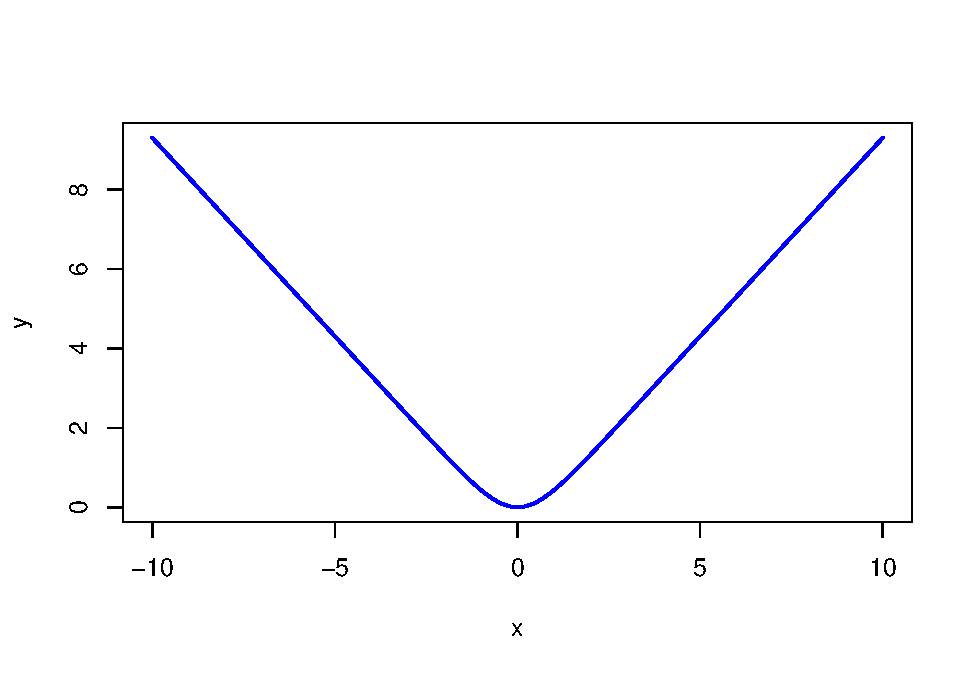
\includegraphics[keepaspectratio]{robust-regression_files/figure-latex/unnamed-chunk-1-1.pdf}}
It is appropriate for a loss function since it is a convex function and
clearly has a global minimum.

\begin{enumerate}
\def\labelenumi{\alph{enumi})}
\setcounter{enumi}{1}
\tightlist
\item
  (1 mark) Write a function of log-cosh loss called \texttt{logcoshfn}.
  \[\rho(\hat{\theta}) = \sum_{u \in \mathcal{P}} \log(\cosh(y_u-\alpha-\beta(x-\bar{x}))) ,\ \theta=(\alpha, \beta)\]
\end{enumerate}

\begin{Shaded}
\begin{Highlighting}[]
\NormalTok{cards }\OtherTok{=} \FunctionTok{read.csv}\NormalTok{(}\StringTok{"data/df\_cards.csv"}\NormalTok{)}

\NormalTok{createlogcoshRho }\OtherTok{\textless{}{-}} \ControlFlowTok{function}\NormalTok{(x, y) \{}
  \DocumentationTok{\#\# local variable}
\NormalTok{  xbar }\OtherTok{\textless{}{-}} \FunctionTok{mean}\NormalTok{(x)}
  \DocumentationTok{\#\# Return this function}
  \ControlFlowTok{function}\NormalTok{(theta) \{ }
\NormalTok{    alpha }\OtherTok{\textless{}{-}}\NormalTok{ theta[}\DecValTok{1}\NormalTok{]}
\NormalTok{    beta }\OtherTok{\textless{}{-}}\NormalTok{ theta[}\DecValTok{2}\NormalTok{]}
    \FunctionTok{sum}\NormalTok{( }\FunctionTok{log}\NormalTok{(}\FunctionTok{cosh}\NormalTok{(y }\SpecialCharTok{{-}}\NormalTok{ alpha }\SpecialCharTok{{-}}\NormalTok{ beta }\SpecialCharTok{*}\NormalTok{ (x }\SpecialCharTok{{-}}\NormalTok{ xbar))) )}
\NormalTok{  \}}
\NormalTok{\}}

\NormalTok{logcoshfn }\OtherTok{=} \FunctionTok{createlogcoshRho}\NormalTok{(cards}\SpecialCharTok{$}\NormalTok{war, cards}\SpecialCharTok{$}\NormalTok{n)}
\end{Highlighting}
\end{Shaded}

\begin{enumerate}
\def\labelenumi{\alph{enumi})}
\setcounter{enumi}{2}
\tightlist
\item
  (3 marks) Find the derivative, write it \textbf{in LaTeX}
\end{enumerate}

\[\frac{d}{dx}\left[ \log(\cosh(x))\right] = \frac{\sinh(x)}{\cosh(x)} = \tanh(x) \]

\[\rho(\hat{\theta}) = \sum_{u \in \mathcal{P}} \log(\cosh(y_u-\alpha-\beta(x-\bar{x}))) ,\ \ \theta=(\alpha, \beta)\]
\[g=\nabla \rho(\theta)=\left[\begin{array}{l}
\frac{d \rho}{d \alpha} \\
\frac{d \rho}{d \beta}
\end{array}\right]=\left[\begin{array}{l}
\sum_{u \in \rho}-\tanh \left(y_u-\alpha-\beta(x-\bar{x})\right) \\
\sum_{u \in \rho}-(x-\bar{x}) \tanh \left(y_u-\alpha-\beta(x-\bar{x})\right)
\end{array}\right]=\left[\begin{array}{l}
\sum_{u \in \rho}-\tanh \left(r_u\right) \\
\sum_{u \in \rho}-(x-\bar{x}) \tanh \left(r_u\right)
\end{array}\right]\]

\begin{enumerate}
\def\labelenumi{\alph{enumi})}
\setcounter{enumi}{3}
\tightlist
\item
  (1 mark) Write a function of the derivative of log-cosh loss called
  \texttt{logcoshprimefn}.
\end{enumerate}

\begin{Shaded}
\begin{Highlighting}[]
\NormalTok{createlogcoshGradient }\OtherTok{\textless{}{-}} \ControlFlowTok{function}\NormalTok{(x, y) \{}
  \DocumentationTok{\#\# local variables}
\NormalTok{  xbar }\OtherTok{\textless{}{-}} \FunctionTok{mean}\NormalTok{(x)}
\NormalTok{  ybar }\OtherTok{\textless{}{-}} \FunctionTok{mean}\NormalTok{(y)}
  \ControlFlowTok{function}\NormalTok{(theta) \{}
\NormalTok{    alpha }\OtherTok{\textless{}{-}}\NormalTok{ theta[}\DecValTok{1}\NormalTok{]}
\NormalTok{    beta }\OtherTok{\textless{}{-}}\NormalTok{ theta[}\DecValTok{2}\NormalTok{]}
\NormalTok{    ru }\OtherTok{=}\NormalTok{ y }\SpecialCharTok{{-}}\NormalTok{ alpha }\SpecialCharTok{{-}}\NormalTok{ beta}\SpecialCharTok{*}\NormalTok{(x }\SpecialCharTok{{-}}\NormalTok{ xbar)}
    \SpecialCharTok{{-}}\DecValTok{1}\SpecialCharTok{*}\FunctionTok{c}\NormalTok{( }\FunctionTok{sum}\NormalTok{(}\FunctionTok{tanh}\NormalTok{(ru)), }
          \FunctionTok{sum}\NormalTok{(}\FunctionTok{tanh}\NormalTok{(ru)}\SpecialCharTok{*}\NormalTok{(x}\SpecialCharTok{{-}}\NormalTok{xbar)) )}
\NormalTok{  \}}
\NormalTok{\}}

\NormalTok{logcoshprimefn }\OtherTok{=} \FunctionTok{createlogcoshGradient}\NormalTok{(cards}\SpecialCharTok{$}\NormalTok{war, cards}\SpecialCharTok{$}\NormalTok{n)}
\end{Highlighting}
\end{Shaded}

\begin{enumerate}
\def\labelenumi{\alph{enumi})}
\setcounter{enumi}{4}
\tightlist
\item
  (5 marks) Use the \texttt{logcoshfn} and \texttt{logcoshprimefn}
  functions as \texttt{rho} and \texttt{gradient} in the
  \texttt{gradientdescent} function, and find a robust estimate of the
  number of cards published (\texttt{n}, y) as a function of the career
  wins above replacement (WAR) (\texttt{war} x) of a baseball player in
  \texttt{df\_cards.csv}, and use it to fit a line to the data and plot
  it. \emph{(Note: WAR is a measure of how much a player has contributed
  to their team's success, compared to a `replacement' player who would
  be someone brought up from a league below. It's possible to have a WAR
  below zero, but in this dataset, those cases have been removed. In
  short, higher WAR means a better player.)}
\end{enumerate}

Use \(\hat\theta_0 = (7,2)\)

\begin{Shaded}
\begin{Highlighting}[]
\NormalTok{gradientDescent }\OtherTok{\textless{}{-}} \ControlFlowTok{function}\NormalTok{(}\AttributeTok{theta =} \DecValTok{0}\NormalTok{,}
\NormalTok{      rhoFn, gradientFn, lineSearchFn, testConvergenceFn,}
      \AttributeTok{maxIterations =} \DecValTok{100}\NormalTok{,}
      \AttributeTok{tolerance =} \FloatTok{1E{-}6}\NormalTok{, }\AttributeTok{relative =} \ConstantTok{FALSE}\NormalTok{,}
      \AttributeTok{lambdaStepsize =} \FloatTok{0.01}\NormalTok{, }\AttributeTok{lambdaMax =} \FloatTok{0.5}\NormalTok{ ) \{}

\NormalTok{  converged }\OtherTok{\textless{}{-}} \ConstantTok{FALSE}
\NormalTok{  i }\OtherTok{\textless{}{-}} \DecValTok{0}

  \ControlFlowTok{while}\NormalTok{ (}\SpecialCharTok{!}\NormalTok{converged }\SpecialCharTok{\&}\NormalTok{ i }\SpecialCharTok{\textless{}=}\NormalTok{ maxIterations) \{}
\NormalTok{    g }\OtherTok{\textless{}{-}} \FunctionTok{gradientFn}\NormalTok{(theta) }\DocumentationTok{\#\# gradient}
\NormalTok{    glength }\OtherTok{\textless{}{-}}  \FunctionTok{sqrt}\NormalTok{(}\FunctionTok{sum}\NormalTok{(g}\SpecialCharTok{\^{}}\DecValTok{2}\NormalTok{)) }\DocumentationTok{\#\# gradient direction}
    \ControlFlowTok{if}\NormalTok{ (glength }\SpecialCharTok{\textgreater{}} \DecValTok{0}\NormalTok{) d }\OtherTok{\textless{}{-}}\NormalTok{ g }\SpecialCharTok{/}\NormalTok{glength}

\NormalTok{    lambda }\OtherTok{\textless{}{-}} \FunctionTok{lineSearchFn}\NormalTok{(theta, rhoFn, d,}
                \AttributeTok{lambdaStepsize =}\NormalTok{ lambdaStepsize, }\AttributeTok{lambdaMax =}\NormalTok{ lambdaMax)}

\NormalTok{    thetaNew }\OtherTok{\textless{}{-}}\NormalTok{ theta }\SpecialCharTok{{-}}\NormalTok{ lambda }\SpecialCharTok{*}\NormalTok{ d}
\NormalTok{    converged }\OtherTok{\textless{}{-}} \FunctionTok{testConvergenceFn}\NormalTok{(thetaNew, theta,}
                                   \AttributeTok{tolerance =}\NormalTok{ tolerance,}
                                   \AttributeTok{relative =}\NormalTok{ relative)}
\NormalTok{    theta }\OtherTok{\textless{}{-}}\NormalTok{ thetaNew}
\NormalTok{    i }\OtherTok{\textless{}{-}}\NormalTok{ i }\SpecialCharTok{+} \DecValTok{1}
\NormalTok{  \}}

  \DocumentationTok{\#\# Return last value and whether converged or not}
  \FunctionTok{list}\NormalTok{(}\AttributeTok{theta =}\NormalTok{ theta, }\AttributeTok{converged =}\NormalTok{ converged, }\AttributeTok{iteration =}\NormalTok{ i, }\AttributeTok{fnValue =} \FunctionTok{rhoFn}\NormalTok{(theta))}
\NormalTok{\}}
\end{Highlighting}
\end{Shaded}

\begin{Shaded}
\begin{Highlighting}[]
\DocumentationTok{\#\#\# line searching could be done as a simple grid search}
\NormalTok{gridLineSearch }\OtherTok{\textless{}{-}} \ControlFlowTok{function}\NormalTok{(theta, rhoFn, d,}\AttributeTok{lambdaStepsize =} \FloatTok{0.01}\NormalTok{, }\AttributeTok{lambdaMax =} \DecValTok{1}\NormalTok{) \{}
  \DocumentationTok{\#\# grid of lambda values to search}
\NormalTok{  lambdas }\OtherTok{\textless{}{-}} \FunctionTok{seq}\NormalTok{(}\AttributeTok{from =} \DecValTok{0}\NormalTok{, }\AttributeTok{by =}\NormalTok{ lambdaStepsize,  }\AttributeTok{to =}\NormalTok{ lambdaMax)}
  \DocumentationTok{\#\# line search}
\NormalTok{  rhoVals }\OtherTok{\textless{}{-}} \FunctionTok{sapply}\NormalTok{(lambdas, }\ControlFlowTok{function}\NormalTok{(lambda) \{}\FunctionTok{rhoFn}\NormalTok{(theta }\SpecialCharTok{{-}}\NormalTok{ lambda }\SpecialCharTok{*}\NormalTok{ d)\})}
  \DocumentationTok{\#\# Return the lambda that gave the minimum}
\NormalTok{  lambdas[}\FunctionTok{which.min}\NormalTok{(rhoVals)]}
\NormalTok{\}}
\end{Highlighting}
\end{Shaded}

\begin{Shaded}
\begin{Highlighting}[]
\DocumentationTok{\#\#\# Where testCovergence might be (relative or absolute)}
\NormalTok{testConvergence }\OtherTok{\textless{}{-}} \ControlFlowTok{function}\NormalTok{(thetaNew, thetaOld, }\AttributeTok{tolerance =} \FloatTok{1E{-}10}\NormalTok{, }\AttributeTok{relative=}\ConstantTok{FALSE}\NormalTok{) \{}
   \FunctionTok{sum}\NormalTok{(}\FunctionTok{abs}\NormalTok{(thetaNew }\SpecialCharTok{{-}}\NormalTok{ thetaOld)) }\SpecialCharTok{\textless{}} \ControlFlowTok{if}\NormalTok{ (relative) tolerance }\SpecialCharTok{*} \FunctionTok{sum}\NormalTok{(}\FunctionTok{abs}\NormalTok{(thetaOld)) }\ControlFlowTok{else}\NormalTok{ tolerance}
\NormalTok{\}}
\end{Highlighting}
\end{Shaded}

\begin{Shaded}
\begin{Highlighting}[]
\FunctionTok{gradientDescent}\NormalTok{(}\AttributeTok{theta =} \FunctionTok{c}\NormalTok{(}\DecValTok{7}\NormalTok{, }\DecValTok{2}\NormalTok{), }\AttributeTok{rhoFn =}\NormalTok{ logcoshfn, }\AttributeTok{gradientFn =}\NormalTok{ logcoshprimefn, }
                \AttributeTok{lineSearchFn =}\NormalTok{ gridLineSearch, }\AttributeTok{testConvergenceFn =}\NormalTok{ testConvergence, }
                \AttributeTok{lambdaStepsize =} \FloatTok{0.001}\NormalTok{)}
\end{Highlighting}
\end{Shaded}

\begin{verbatim}
## $theta
## [1] 5.1895266 0.1694879
## 
## $converged
## [1] TRUE
## 
## $iteration
## [1] 70
## 
## $fnValue
## [1] 6431.333
\end{verbatim}

\begin{Shaded}
\begin{Highlighting}[]
\FunctionTok{plot}\NormalTok{(cards}\SpecialCharTok{$}\NormalTok{n, cards}\SpecialCharTok{$}\NormalTok{war)}
\FunctionTok{abline}\NormalTok{(}\DecValTok{7}\NormalTok{, }\DecValTok{2}\NormalTok{)}
\FunctionTok{abline}\NormalTok{(}\FloatTok{5.1895266}\NormalTok{, }\FloatTok{0.1694879}\NormalTok{, }\AttributeTok{col =} \StringTok{"blue"}\NormalTok{)}
\end{Highlighting}
\end{Shaded}

\pandocbounded{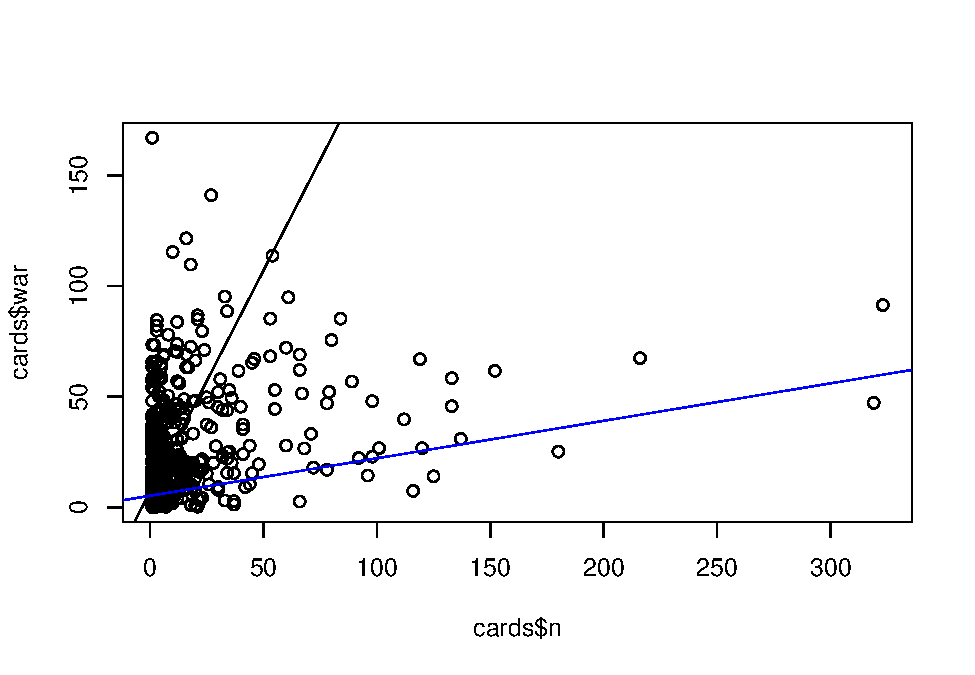
\includegraphics[keepaspectratio]{robust-regression_files/figure-latex/unnamed-chunk-7-1.pdf}}

\begin{enumerate}
\def\labelenumi{\alph{enumi})}
\setcounter{enumi}{5}
\tightlist
\item
  (1 mark) Check your work using the \texttt{optim} function with the
  same initial values for \texttt{par} and \texttt{rho} as the
  \texttt{fn}.
\end{enumerate}

\begin{Shaded}
\begin{Highlighting}[]
\FunctionTok{optim}\NormalTok{(}\AttributeTok{par=}\FunctionTok{c}\NormalTok{(}\DecValTok{7}\NormalTok{, }\DecValTok{2}\NormalTok{), }\AttributeTok{fn =}\NormalTok{ logcoshfn)}
\end{Highlighting}
\end{Shaded}

\begin{verbatim}
## $par
## [1] 5.176915 0.168554
## 
## $value
## [1] 6431.324
## 
## $counts
## function gradient 
##       71       NA 
## 
## $convergence
## [1] 0
## 
## $message
## NULL
\end{verbatim}

\end{document}
